\begin{figure}[H]
    \centering
    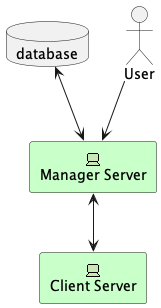
\includegraphics[height=0.4\textheight]{./part/Proyecto_ejecutivo/memoria_descriptiva/descripcionDelProyecto/manager/uml/managerServerConcept}
    \caption{Diagrama UML de despliegue del manager}\label{fig:diagrama_uml_de_despliegue_del_manager}
\end{figure}

Podemos apreciar en el diagrama UML de desplique~\cref{fig:diagrama_uml_de_despliegue_del_manager} que el programa Manager será el programa conel que interactue directamente el usuario para transferir sus comandos al programa Cliente y que dispondrá de una base de datos para almacenar de forma persistente toda la información necesaria.

\subparagraph{Dominio}

\begin{figure}[H]
    \centering
    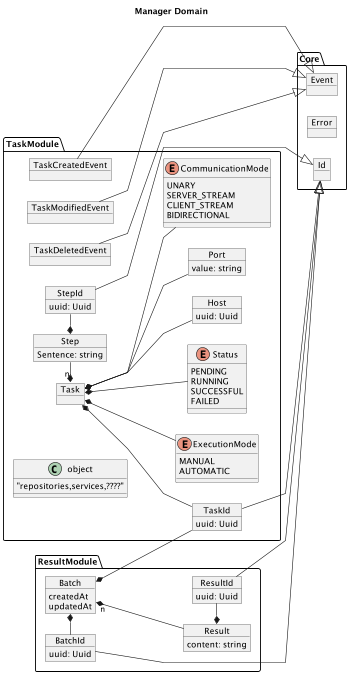
\includegraphics[height=0.4\textheight]{./part/Proyecto_ejecutivo/memoria_descriptiva/descripcionDelProyecto/manager/uml/managerDomain}
    \caption{Diagrama UML de el dominio de manager}\label{fig:Diagrama UML de el dominio de manager}
\end{figure}

En el diagrama UML~\cref{fig:Diagrama UML de el dominio de manager} vemos que el dominio de Manager se compone de dos modulos: uno para las tareas, Task; otro para los resultados, Result; y otro Core para los elementos básicos del sistema que comparte toda el Dominio:
\begin{itemize}
    \item CoreDomain
        \begin{itemize}
            \item \textbf{Id}: todos los ids extienden de el, para no reescribir código. contiene un \textit{UUID}, el paquete para generarlos habrá que seleccionarlo según los que nos ofrece el ecosistema. Es la única dependencia externas que vamos a tener dentro del dominio por ello la encapsulamos en el paquete core para no dispersar a lo largo de todo el Domino dicha dependencia, por si hubiese que cambiarla.
            \item Event todos los eventos del sistema extenderan de él
        \end{itemize}
    \item TaskDomain
        \begin{itemize}
        \item \textbf{Task}: AggregateRoot
        \item \textbf{TaskId}: cada Entidad tiene su Id tipo, para evitar errores. Si usaramos el mismo tipo Id para todas, cuando buscaras una Task mediante un Id que corresponde a un Result estaría correctamente tipado pero sería incorrecto, no lo encontraríamos, pero no nos advertiría de nuestro error
        \item \textbf{Host}: es un \textit{Value Object} compuesto por el valor del host, es un string pero el \textit{Value Object} garantiza que es un valor válido, si no devuelve un error
        \item \textbf{Port}: es un \textit{Value Object} compuesto por el valor del puerto, es un string pero el \textit{Value Object} garantiza que es un valor válido, si no devuelve un error
        \item \textbf{CommunicationMode}: es un Enum para expresar esa tarea de las formas de comunicación posibles que hay entre dos servidores cual sera la utilizada
            \begin{itemize}
                \item UNARY
                \item SERVER\_STREAM
                \item CLIENT\_STREAM
                \item BIDIRECTIONAL
            \end{itemize}
        \item \textbf{ExecutionMode}: es un enum para expresar los modos de ejecución
        \begin{itemize}
            \item MANUAL
            \item AUTOMATIC
        \end{itemize}
        \item \textbf{Status}: es un enum \label{taskStatus}
        \begin{itemize}
            \item PENDING
            \item RUNNING
            \item SUCCESSFUL
            \item FAILED
        \end{itemize}
        \item \textbf{Step}: cada tarea puede componerse en distintos pasos. Por ejemplo queremos poder poner en marcha el motor durante 15 segudos y luego llevarlo a una posición de inicio
        \begin{itemize}
            \item \textbf{StepId}
            \item \textbf{sentence}: string de contenido libre que el servidor que contiene el programa cliente ejecutará. Depende del gestor del servidor de él dicho programa que el programa cliente quiere ejecutar se encuentre instalado
        \end{itemize}
        \item \textbf{TaskCreatedEvent}: cuando se cree una tarea se emitirá un evento, habrá un manejador de eventos que actuará en consecuencia. Si es una tarea automatizada y el loop de ejecución está parado lo pondrá en marcha.
        \item \textbf{TaskModifiedEvent}: evento emitido cuando una tarea es modificada habrá un manejador de eventos que actuará en consecuencia. Si la tarea vuelve a ser puesta a pending, es automatizada y el loop de ejecución está parado lo pondrá en marcha
    \end{itemize}
    \item \textbf{ResultDomain}
        \begin{itemize}
            \item \textbf{BatchId}
            \item \textbf{Batch}: \textit{Agreggate Root} para referencial el conjunto de resultados correspondiente a la ejecución de una tarea. Una tarea no sólo se puede ejecutar varias veces, cada vez con distintos resultados, si no que además para una ejecución pueden obtenerse también varios resultados. Para identificarlos y agruparlos necesitaremos este \textit{Agreggate Root}.
            \item \textbf{ResultId}
            \item \textbf{Result}: String con el resultado en plano. Cada tarea y proceso tendrá a su disposición este strings para crear su propio formato de respuesta. Será tarea de cada cliente interpretarlos.
        \end{itemize}
\end{itemize}

\subparagraph{Casos de uso}

En el Manager Tenemos 2 Entities y dos \textit{Agreggate Root}, sobre ellos serán los casos de uso con los que podrá interactuar el usuario.

\begin{itemize}
    \item Task
    \subitem Step
    \item Batch
    \subitem Result
\end{itemize}

Vamos a hacer el \gls{CRUD} completo de Task, dentro de éste, se contempla la edición de los steps a través de Task ya que es su \textit{Agreggate Root} y por definición no se debe poder acceder a sus componentes si no es a través del \textit{Agreggate Root}. De Batch y Result no vamos a permitir el update por lógica de dominio este caso de uso no debe existir, ya que sus variables son autogeneradas en el momento de creación.

\textbf{Create Task}

La lógica de crear tareas se basará en la comprobación de que la información de entrada es correcta y suficiente, es decir, no hay parámetros opcionales. Por lo tanto deberán estar todos y ser validos. Esto se hará en la instanciación de los \textit{Value Object}. Si alguno de los datos no es válido el flujo se detendrá, devolviendo el error corespondiente al usario para que pueda subsanarlo y enviar una nueva petición.

\begin{figure}[H]
    \centering
    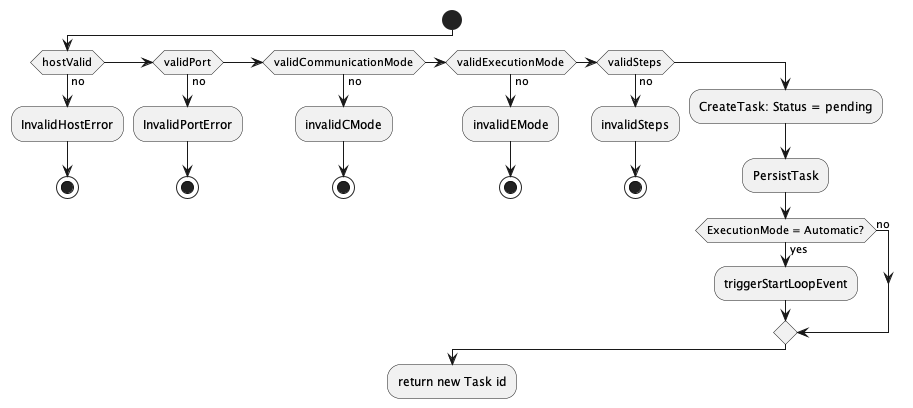
\includegraphics[height=0.2\textheight]{./part/Proyecto_ejecutivo/memoria_descriptiva/descripcionDelProyecto/manager/uml/createTaskUseCase}
    \caption{Use Case: Create Task}\label{fig:Use Case-Create Task}
\end{figure}

\textbf{Read Task}

La obtención de una Task se hará a través de su identificador \textit{UUID}. Se comprobará que efectivamente existe una Task con dicho identificador y de se devolverá el resultado de dicha búsqueda.

\begin{figure}[H]
    \centering
    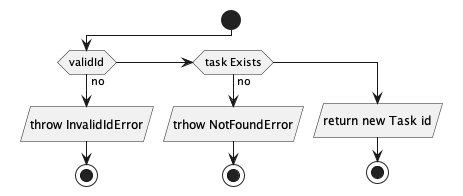
\includegraphics[height=0.15\textheight]{./part/Proyecto_ejecutivo/memoria_descriptiva/descripcionDelProyecto/manager/uml/getTaskUseCase}
    \caption{Use Case: Read Task}\label{fig:Use Case-Read Task}
\end{figure}

\textbf{Read Tasks}

Uno de los puntos más amplios en una \textit{API CRUD} es el filtrado de datos. No entra dentro del ámbito de este proyecto crear un sistema de filtrado que incluya la paginación. En este caso habría que crear una nomenclatura de filtros de cara al usuario y un sistema que los procese, devolviendo error ante un filtro erroneo o el listado de tareas que responda a dicho filtro. En nuestro caso devolveremos todas las tareas.

\textbf{Update Task}

A diferencia del flujo de creación en este caso si ha parámetros opcionales. Ya que este flujo equivale a lo que en \gls{REST} se entiende como \textit{PATCH}, es decir una actualización parcial, los parámetros que no se reciban en la petición quedarán intactos. En un PUT el parámetro que no se recive se entiende que ha de ser eliminado.

\begin{figure}[H]
    \centering
    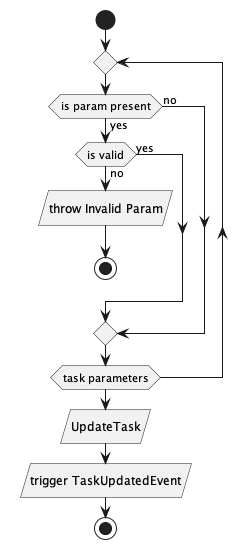
\includegraphics[height=0.4\textheight]{./part/Proyecto_ejecutivo/memoria_descriptiva/descripcionDelProyecto/manager/uml/updateTaskUseCase}
    \caption{Use Case: Update Task}\label{fig:Use Case-Update Task}
\end{figure}

\textbf{Delete Task}

En el flujo de eliminación de tareas, además de confirmar que la tarea que se desea eliminar existe, se añadirán más validaciones para garantizar al consistencia del sistema. No se permitirán eliminar tareas que estén en status \textit{RUNNING}

\begin{figure}[H]
    \centering
    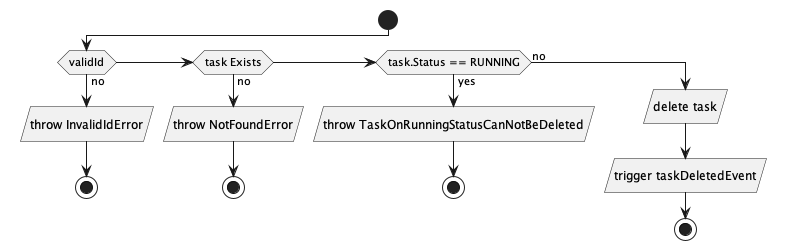
\includegraphics[height=0.2\textheight]{./part/Proyecto_ejecutivo/memoria_descriptiva/descripcionDelProyecto/manager/uml/deleteTaskUseCase}
    \caption{Use Case: Delete Task}\label{fig:Use Case-Delete Task}
\end{figure}

\textbf{TaskEventHandler}

Tanto en \textit{TaskCreatedEvent} como \textit{TaskUpdatedEvent} el handler va a ser el mismo. El gestor de eventos~\cref{fig:Use Case-TaskEventHandler} comprobará si la tarea es de tipo \textit{AUTOMATIC}, o se ha modificado a ese tipo. Comprobará si se acaba de crear, y por lo tanto el status es \textit{PENDING}, o se ha modificado a dicho tipo. Si las dos primeras condiciones se cumplen entonces comprobará que el loop de gestión de tareas está habilitado; de no ser así se habilitará.

\begin{figure}[H]
    \centering
    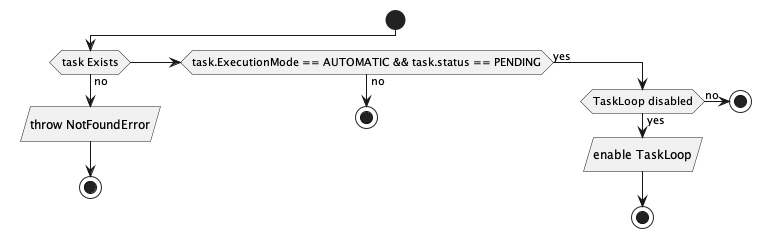
\includegraphics[height=0.2\textheight]{./part/Proyecto_ejecutivo/memoria_descriptiva/descripcionDelProyecto/manager/uml/taskEventHandlerUseCase}
    \caption{Use Case: TaskEventHandler}\label{fig:Use Case-TaskEventHandler}
\end{figure}

\textbf{TaskLoop: ejecutar tareas automáticas}\label{ref:X}

Cuando \textit{TaskEventHandler} pone en marcha el \textit{TaskLoop} este obtendrá de base de datos todas las tareas automáticas pendientes y iterando sobre ellas lanzará un hilo de ejecución para ejecutarlas. Una vez terminadas todas volverá a intentar obtener tareas pendientes ya que en el periodo que haya estado ejecutandolas pueden haberse introducido nuevas. Si no hay más tareas pendientes el loop se desactivará.

En este caso de uso es el core de la aplicación, donde se pondrá en juego la asincronía y todo el potencial del lenguaje. Es por tanto una primera versión del diseño. Igual que los otros casos de uso son lógica rutinaria que no debiera diferir mucho del diseño original, en este caso sí que podemos encontrarnos con lógicas que no estén previstas y por lo tanto haya que modificar. Todo quedará reflejado en la memoria explicativa de cambios~\cref{subsec:memoria explicativa de cambios}.

\begin{figure}[H]
    \centering
    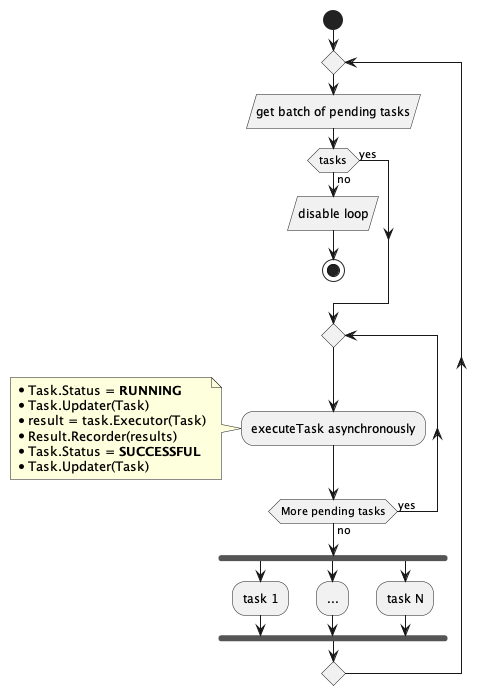
\includegraphics[height=0.4\textheight]{./part/Proyecto_ejecutivo/memoria_descriptiva/descripcionDelProyecto/manager/uml/executeTaskLoop}
    \caption{Use Case: TaskLoop}\label{fig:Use Case-TaskLoop}
\end{figure}

Atendiendo por tanto a esta posibilidad de cambio se hará uso de la arquitectura para desacoplarnos de dicha incertidumbre \textbf{TaskProcessor} que aparece en la figura~\cref{fig:Use Case-TaskLoop} en color verde es el proceso asíncrono donde se hará uso del las gorutines que permiten la gestión de tareas asíncronas de forma sencilla. Lo definiremos como un puerto de salida e implementaremos un adaptador para encapsular esa incertidumbre.

Es de preveer que dentro de ese adaptador se implemente lógica que habrá de ser de negocio. Sin embargo, a no poder vislumbrarla con claridad, preferimos dejar pendiente de una refactorización. La refactorización posterior podrá ir introduciendo en dominio y limpiando dicho adaptador de el posible mal código resultado de la investigación mientras se construye, en vez de ensuciar el dominio y acoplar nuestro código base a esta incertidumbre.

A pesar de dicho desconocimiento inicial que nos impide diseñar con exactitud el flujo, El objetivo de este proyecto ejecutivo es hacer siempre una primera iteración en la medida que se pueda. Por lo tanto una primera iteración se puede ver en la figura~\cref{fig:Use Case-Task Processor}

\begin{figure}[H]
    \centering
    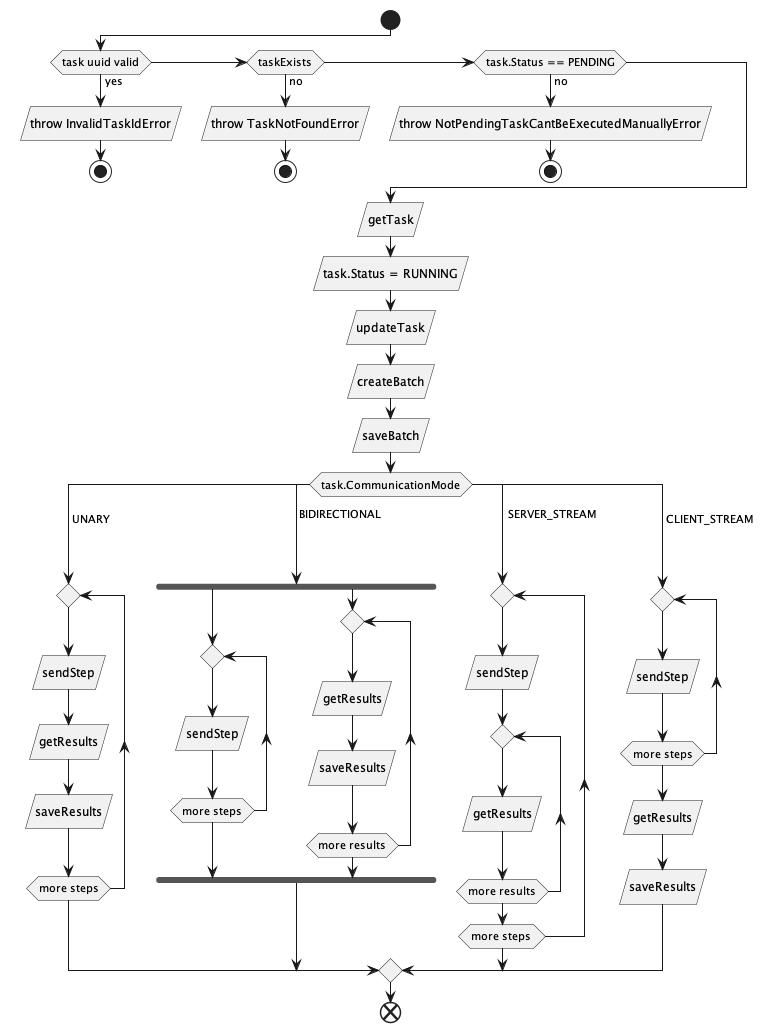
\includegraphics[height=0.55\textheight]{./part/Proyecto_ejecutivo/memoria_descriptiva/descripcionDelProyecto/manager/uml/1-TaskProcessor}
    \caption{Use Case: Task Processor}\label{fig:Use Case-Task Processor}
\end{figure}

Podemos ver que está muy acoplado a la interacción de los flujos de comunicación \textit{RPC}~\cref{subsubsec:communications} de ahí nuestra incertidumbre al no haber trabajado todavía con dicha tecnología.

\textbf{Create Batch}

\begin{figure}[H]
    \centering
    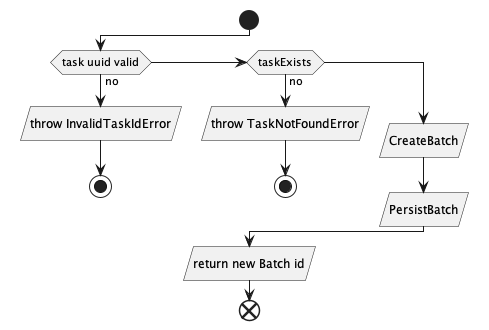
\includegraphics[height=0.2\textheight]{./part/Proyecto_ejecutivo/memoria_descriptiva/descripcionDelProyecto/manager/uml/createBatchUseCase}
    \caption{Use Case: Create Batch}\label{fig:Use Case: Create Batch}
\end{figure}

\textbf{Delete Batch}

\begin{figure}[H]
    \centering
    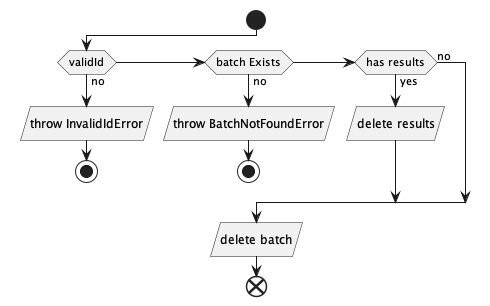
\includegraphics[height=0.2\textheight]{./part/Proyecto_ejecutivo/memoria_descriptiva/descripcionDelProyecto/manager/uml/deleteBatchUseCase}
    \caption{Use Case: Delete Batch}\label{fig:Use Case: Delete Batch}
\end{figure}

\textbf{Read batch}

\begin{figure}[H]
    \centering
    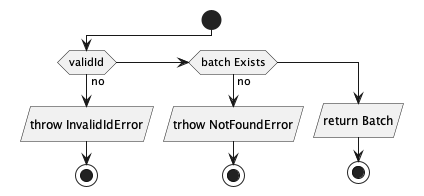
\includegraphics[height=0.2\textheight]{./part/Proyecto_ejecutivo/memoria_descriptiva/descripcionDelProyecto/manager/uml/getBatchUseCase}
    \caption{Use Case: Read Batch}\label{fig:Use Case: Read Batch}
\end{figure}

\textbf{Read batches of a Task}

\begin{figure}[H]
    \centering
    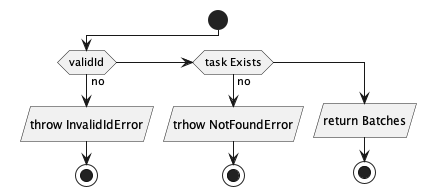
\includegraphics[height=0.2\textheight]{./part/Proyecto_ejecutivo/memoria_descriptiva/descripcionDelProyecto/manager/uml/getTaskBatchUseCase}
    \caption{Use Case: Read Batches of Task}\label{fig:Use Case-Read Batches of Task}
\end{figure}

\textbf{Obtener los results de un batch}

\begin{figure}[H]
    \centering
    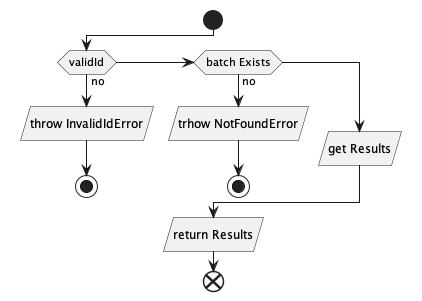
\includegraphics[height=0.2\textheight]{./part/Proyecto_ejecutivo/memoria_descriptiva/descripcionDelProyecto/manager/uml/getBatchResultsUseCase}
    \caption{Read Results of a Batch Use Case}\label{fig:Read Results of a Batch Use Case}
\end{figure}

\textbf{Execute task manually}

Solo se puede ejecutar una tarea manual por vez, en este primer diseño. El motivo es que como se quiere graficar en tiempo real la respuesta, por ejemplo para monitorizar la velocidad del motor en tiempo real, no queremos meternos en la complejidad de graficar varios resultados a la vez.

\begin{figure}[H]
    \centering
    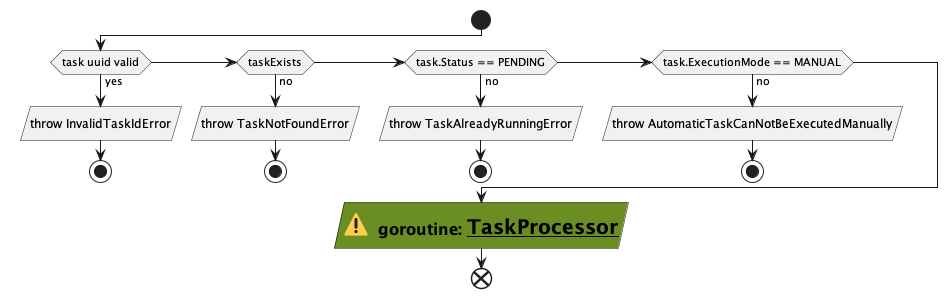
\includegraphics[height=0.2\textheight]{./part/Proyecto_ejecutivo/memoria_descriptiva/descripcionDelProyecto/manager/uml/1-executeTaskManual}
    \caption{Use Case: Execute Task Manually}\label{fig:Use Case-Execute Task Manually}
\end{figure}

El diagrama de secuencia para el caso de que una tarea sea de tipo \textit{BIDIRECTIONAL} se puede apreciar en el diagrama~\cref{fig:executeTaskManualInteraction}. Este es el caso que utilizaremos por ejemplo para el control en velocidad y posición del motor de corriente continua. Se enviará una consigna y se recibirán resultados hasta que el cliente envíe la orden de detener dicho control. Para otros tipos más simples, por ejemplo, ejecutar manualmente la tarea de configurar el PID, simplemente será de tipo \textit{UNARY}, se enviará una request y se obtendrá una respuesta.

\begin{figure}[H]
    \centering
    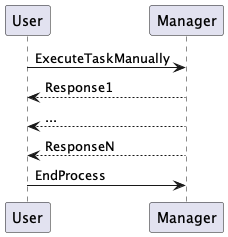
\includegraphics[height=0.2\textheight]{./part/Proyecto_ejecutivo/memoria_descriptiva/descripcionDelProyecto/manager/uml/1-ExecuteTaskManuallyInteraction}
    \caption{Execute task manually interaction}\label{fig:executeTaskManualInteraction}
\end{figure}

\subparagraph{estructura de carpetas}

Una de las partes mas importantes de un proyecto de software es que la estructura de carpetas hable sobre cómo está diseñado el software. Cuando alguien entra en un proyecto tener que entrar a los archivos y leer código para hacerse una idea general no es intuitivo. La estructura de carpetas debe expresar la arquitectura con la que está diseñada. Los nombres de los archivos debe expresar lo que contienen. Hacer fácil el autodescubrimiento y encontrar lo que se esté buscando. Cada lenguaje, framework o comunidad tienen sus propios estándares. Nosotros vamos a seguir el que sugiere~\cite{TomHombergs2019GYHD}. Que expresa con claridad que estamos ante una arquitectura hexagonal, o de puertos y adaptadores y que el Dominio se encuentra estructurado mediante un diseño \textit{DDD} expresando el \textit{UL} en los propios nombres de los archivos.

En el proyecto constará de 4 carpetas principales
\dirtree{%
    .1 Project .
        .2 Adapter.
        .2 Application.
        .2 Domain.
        .2 Bootstrap.
}

Bootstrap será donde hagamos la composición de la aplicación, es decir la inyección de dependencias.

Vamos a desplegar la estructura capa por capa

\textbf{Adapters}

\dirtree{%
.1 Adapter.
    .2 in.
        .3 GRPC.
            .4 CreateEntityGrpcCall.
        .3 Console.
            .4 CreateEntityTerminalCommand.
    .2 out.
        .3 Email.
            .4 SendEmailOnCreationImplementation (*1).
        .3 Mysql.
            .4 SaveEntityImplementation (*2).
}

\textbf{Aplicación}

\dirtree{%
.1 Application.
    .2 Port.
        .3 in.
            .4 Entity.
                .5 CreateUseCase.
                    .6 CreateCommand.
                        .7 CreateCommand (using sendEmail param in this example).
                        .7 CreateUseCase.
                    .6 SomeEventHandler.
                        .7 CreationEvent.
                        .7 CreationEventUseCase.
        .3 out.
            .4 Email.
                .5 SendEmailConCreation (interface for *1).
}

\textbf{Dominio}

\dirtree{%
.1 Domain.
    .2 Core.
        .3 Id.
        .3 Event.
        .3 Error.
    .2 Task.
        .3 Id.
        .3 Task.
        .3 Host.
        .3 Port.
        .3 CommunicationMode.
        .3 ExecutionMode.
        .3 Status.
        .3 Step.
            .4 Id.
            .4 StepEntity.
            .4 StepVo.
            .4 Repository.
                .5 Find.
                .5 Save.
                .5 Search.
                .5 Delete.
                .5 Update.
            .4 Service.
                .5 Finder.
                .5 Creator.
                .5 Updater.
                .5 Eraser.
                .5 Searcher.
        .3 Repository.
            .4 Find.
            .4 Save.
            .4 Search.
            .4 Delete.
            .4 Update.
        .3 Service.
            .4 Finder.
            .4 Creator.
            .4 Updater.
            .4 Eraser.
            .4 Searcher.
    .2 Result.
}

